\actTitle{2.1 Part 1 - Quadratic Functions and Applications}

\videoLink{Section 2.1 Day 1}{https://www.youtube.com/playlist?list=PLYHZK3b8UFw1r2QdO6Pgj4jg4-OBM6h1I}

\noindent \textbf{Topics:}  quadratic functions, standard equation for  a quadratic, and vertex of a parabola\\

\noindent \textbf{Student Learning Outcomes:}
\begin{enumerate}
\item Students will be able to recognize quadratic functions graphically and algebraically.
\item Students will be able to write the standard equation for a quadratic function.
\item Students will be able to determine the vertex of a parabola.
\end{enumerate}

\hrule 

\bigskip

\subsection{Standard Form of a Quadratic Function} ~

\noindent \underline{Quadratic Formula.} The roots of the equation $ax^2+bx+c=0$ are \\
\begin{eqnarray}
  x = \dfrac{-b \pm \sqrt{b^2-4ac}}{2a}
\end{eqnarray}

\hspace{-.3in}\begin{tabular}{| p{0.8\textwidth} |} \hline 
\noindent \underline{Standard Equation of a Parabola.}
The standard equation of a parabola is 
$ y = a(x-h)^2 + k$. The point $(h,k)$ is the vertex of the parabola.
\\ \hline
\end{tabular} 

      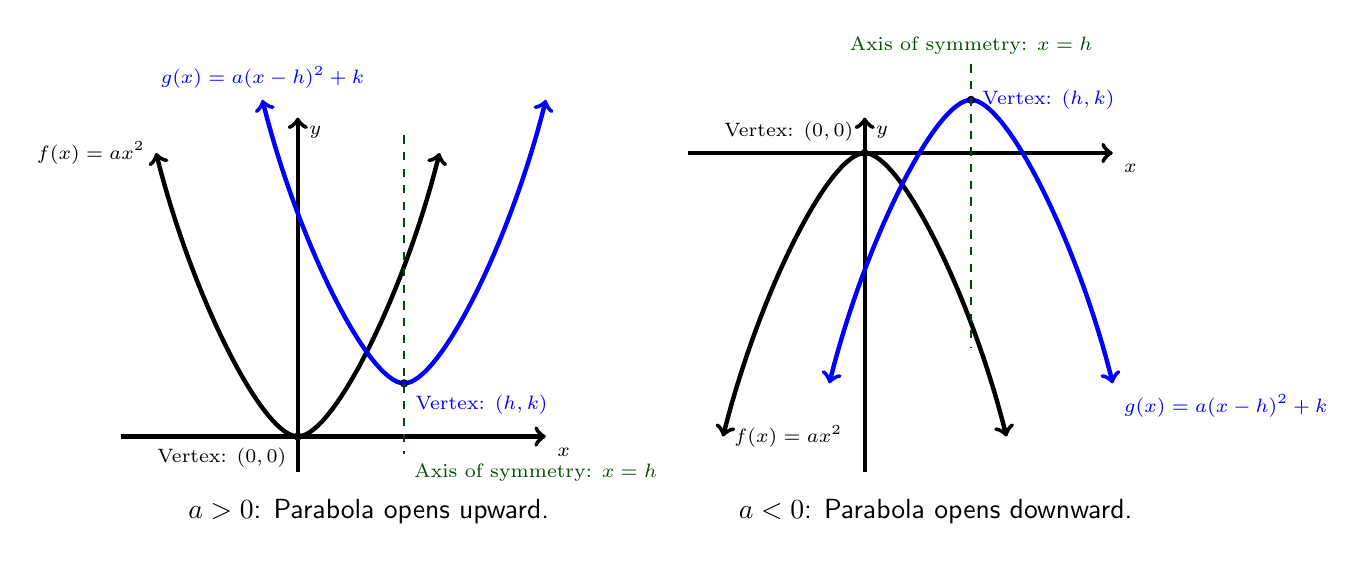
\begin{tikzpicture}[y=0.9cm, x=0.9cm,font=\sffamily]
        \begin{scope} %[shift={(0,8)}]
           \draw[ultra thick,->] (-2.5,0) -- coordinate (x axis mid) (3.5,0)
                node[font=\scriptsize,anchor = north west] {$x$}; 
           \draw[ultra thick,->] (0,-0.5) -- coordinate (y axis mid) (0,4.5) 
                node[font=\scriptsize,anchor = west,shift={(0.0,-0.2)}]  {$y$};
        \end{scope}
        \begin{scope} %[shift={(0,8)}]
           \draw[ultra thick,black,<-]
           (-2,4) .. controls +( 0.5,-2) and +(-0.5, 0) .. (0,0)
           node[font=\scriptsize,anchor=east,pos=0] {$f(x)=ax^2$};
           \draw[ultra thick,black,->]
           ( 0,0) .. controls +( 0.5, 0) and +(-0.5,-2) .. (2,4)
           node[font=\scriptsize,anchor=north east,pos=0] {Vertex: $(0,0)$};
           \draw[fill=black]  (0,0) circle (0.05);
         \end{scope}
        \begin{scope}[shift={(1.5,0.75)}]
           \draw[ultra thick,blue,<-]
           (-2,4) .. controls +( 0.5,-2) and +(-0.5, 0) .. (0,0)
           node[font=\scriptsize,anchor=south,pos=0,blue] {$g(x)=a(x-h)^2+k$};
           \draw[ultra thick,blue,->]
           ( 0,0) .. controls +( 0.5, 0) and +(-0.5,-2) .. (2,4)
           node[font=\scriptsize,anchor=north west,pos=0] {Vertex: $(h,k)$};
           \draw[fill=blue]  (0,0) circle (0.05);
           \draw[thick,dashed,green!30!black] (0,3.5) -- (0,-1)
           node[font=\scriptsize,anchor=north west,green!30!black] {Axis of symmetry: $x=h$};
           \node[black,anchor=north,shift={(-0.5,0)}] at (0,-1.5) {$a>0$: Parabola opens upward.};
         \end{scope}

        \begin{scope}[shift={(8,4)}]
           \draw[ultra thick,->] (-2.5,0) -- coordinate (x axis mid) (3.5,0)
                node[font=\scriptsize,anchor = north west] {$x$}; 
           \draw[ultra thick,->] (0,-4.5) -- coordinate (y axis mid) (0,0.5) 
                node[font=\scriptsize,anchor = west,shift={(0.0,-0.2)}]  {$y$};
        \end{scope}
        \begin{scope}[shift={(8,4)}]
           \draw[ultra thick,black,<-]
           (-2,-4) .. controls +( 0.5,2) and +(-0.5, 0) .. (0,0)
           node[font=\scriptsize,anchor=west,pos=0] {$f(x)=ax^2$};
           \draw[ultra thick,black,->]
           ( 0,0) .. controls +( 0.5, 0) and +(-0.5,2) .. (2,-4)
           node[font=\scriptsize,anchor=south east,pos=0] {Vertex: $(0,0)$};
           \draw[fill=black]  (0,0) circle (0.05);
         \end{scope}
        \begin{scope}[shift={(9.5,4.75)}]
           \draw[ultra thick,blue,<-]
           (-2,-4) .. controls +( 0.5,2) and +(-0.5, 0) .. (0,0);
           \draw[ultra thick,blue,->]
           ( 0,0) .. controls +( 0.5, 0) and +(-0.5,2) .. (2,-4)
           node[font=\scriptsize,anchor=west,pos=0] {Vertex: $(h,k)$}
           node[font=\scriptsize,anchor=north west,pos=1,blue] {$g(x)=a(x-h)^2+k$};
           \draw[fill=blue]  (0,0) circle (0.05);
           \draw[thick,dashed,green!30!black] (0,0.5) -- (0,-3.5)
           node[font=\scriptsize,anchor=south,green!30!black,pos=0] {Axis of symmetry: $x=h$};
           \node[black,anchor=north,shift={(-0.5,0)}] at (0,-5.5) {$a<0$: Parabola opens downward.};
         \end{scope}

        \end{tikzpicture}


\newpage


\subsection{Graphing a Quadratic Function in Standard Form}

\begin{enumerate}
\item The graph of a quadratic function is given.  Select the function's equation.\\
\includegraphics[scale=.7]{quad1a}\includegraphics[scale=.7]{quad1b}\\
\item Given $f(x)=-2(x-1)^2+8$
\begin{enumerate}
\item Determine whether the graph of the parabola opens upward or downward.\\[.3in]
\item Identify the vertex.\\[.3in]
\item Determine the $x$-intercept(s).\\[1in]
\item Determine the $y$-intercept.\\[.5in]

\clearpage

\item Sketch the function.

      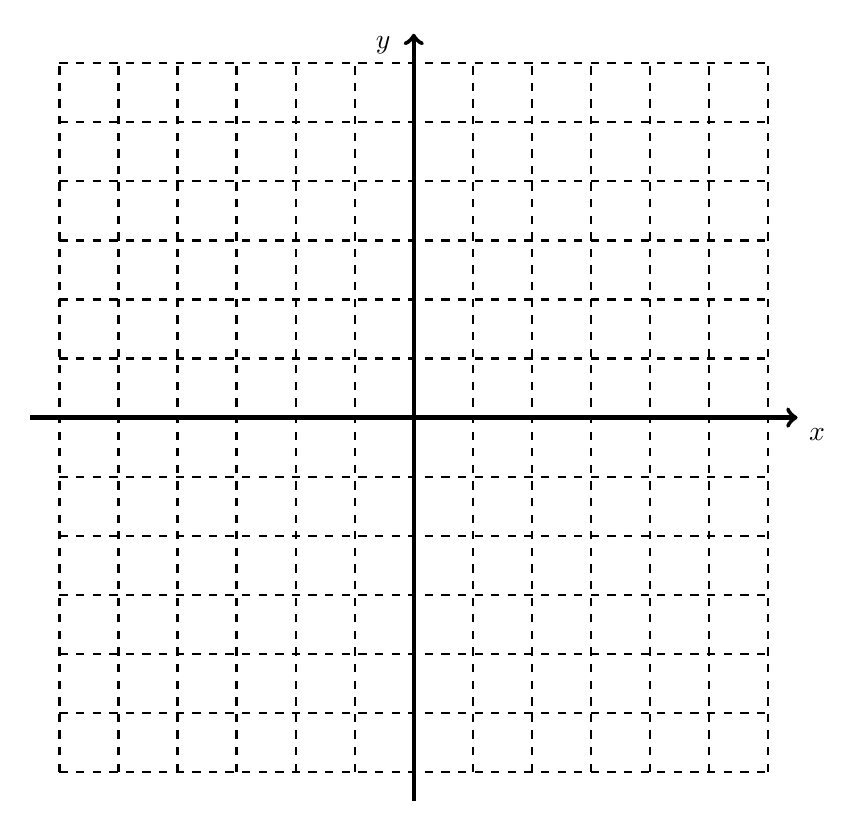
\begin{tikzpicture}[y=0.75cm, x=0.75cm,font=\sffamily]
        \begin{scope} %[shift={(0,8)}]
          %% ticks
          \draw[xstep = 1, ystep=1.0,black,dashed,thick] % very thin,opacity=0.85,
                 (-6.0,-6.0) grid ( 6.0, 6.0);
             %% axis
           \draw[ultra thick,->] (-6.5,0) -- coordinate (x axis mid) (6.5,0)
                node[anchor = north west] {$x$}; 
           \draw[ultra thick,->] (0,-6.5) -- coordinate (y axis mid) (0,6.5) 
                node[anchor = east,shift={(-0.2,-0.2)}]  {$y$};

           %\foreach \y in {-1,1,...,4} {
           %   \draw (1pt, \y) -- (-1pt, \y) node[yshift=-6,xshift=1,anchor=west] {$\y$};
           % }
           %\foreach \x in {-3,-2,-1,1,2,3} {
           %   \draw (\x,1pt) -- (\x,-1pt) node[yshift=-5,xshift=-1,anchor=east] {$\x$};
           % }

          \end{scope}
        \end{tikzpicture}


\item Determine the axis of symmetry.\\



\end{enumerate}






\newpage



\subsection{Determining the Standard Form of Quadratic Function}

\noindent To determine the standard form of a quadratic function written in the form $y=ax^2+bx+c$, we use a process called \textbf{Completing the Square}.


 
 \item Determine the standard equation of the parabola $y=3x^2+12x+5$.  Then determine the vertex.
 
 
 \vfill
 
  
 \includegraphics[scale=.75]{parabola}






\end{enumerate}

\noindent \textbf{Student Learning Outcomes Check}

\begin{enumerate}
\item Are you able to recognize quadratic functions graphically and algebraically?
\item Can you write the standard equation for a quadratic function?
\item Are you able to determine the vertex of a parabola?


\end{enumerate}

\noindent \textbf{If any of your answers were no, please ask about these topics in class.}


